\documentclass{article}
\usepackage[utf8]{inputenc}
\usepackage[export]{adjustbox}
\usepackage{subfigure}
\usepackage{url}
\usepackage{graphicx}
\graphicspath{
	{images/}
}

\begin{document}

\title{Design Ideas}
\author{Cardspark - Group 26}
\date{\today}
\maketitle 

We had the idea of a revision app due to our previous difficulties in revision so we choose to research this idea with our peers.

\begin{center}
	\vspace{1mm}
	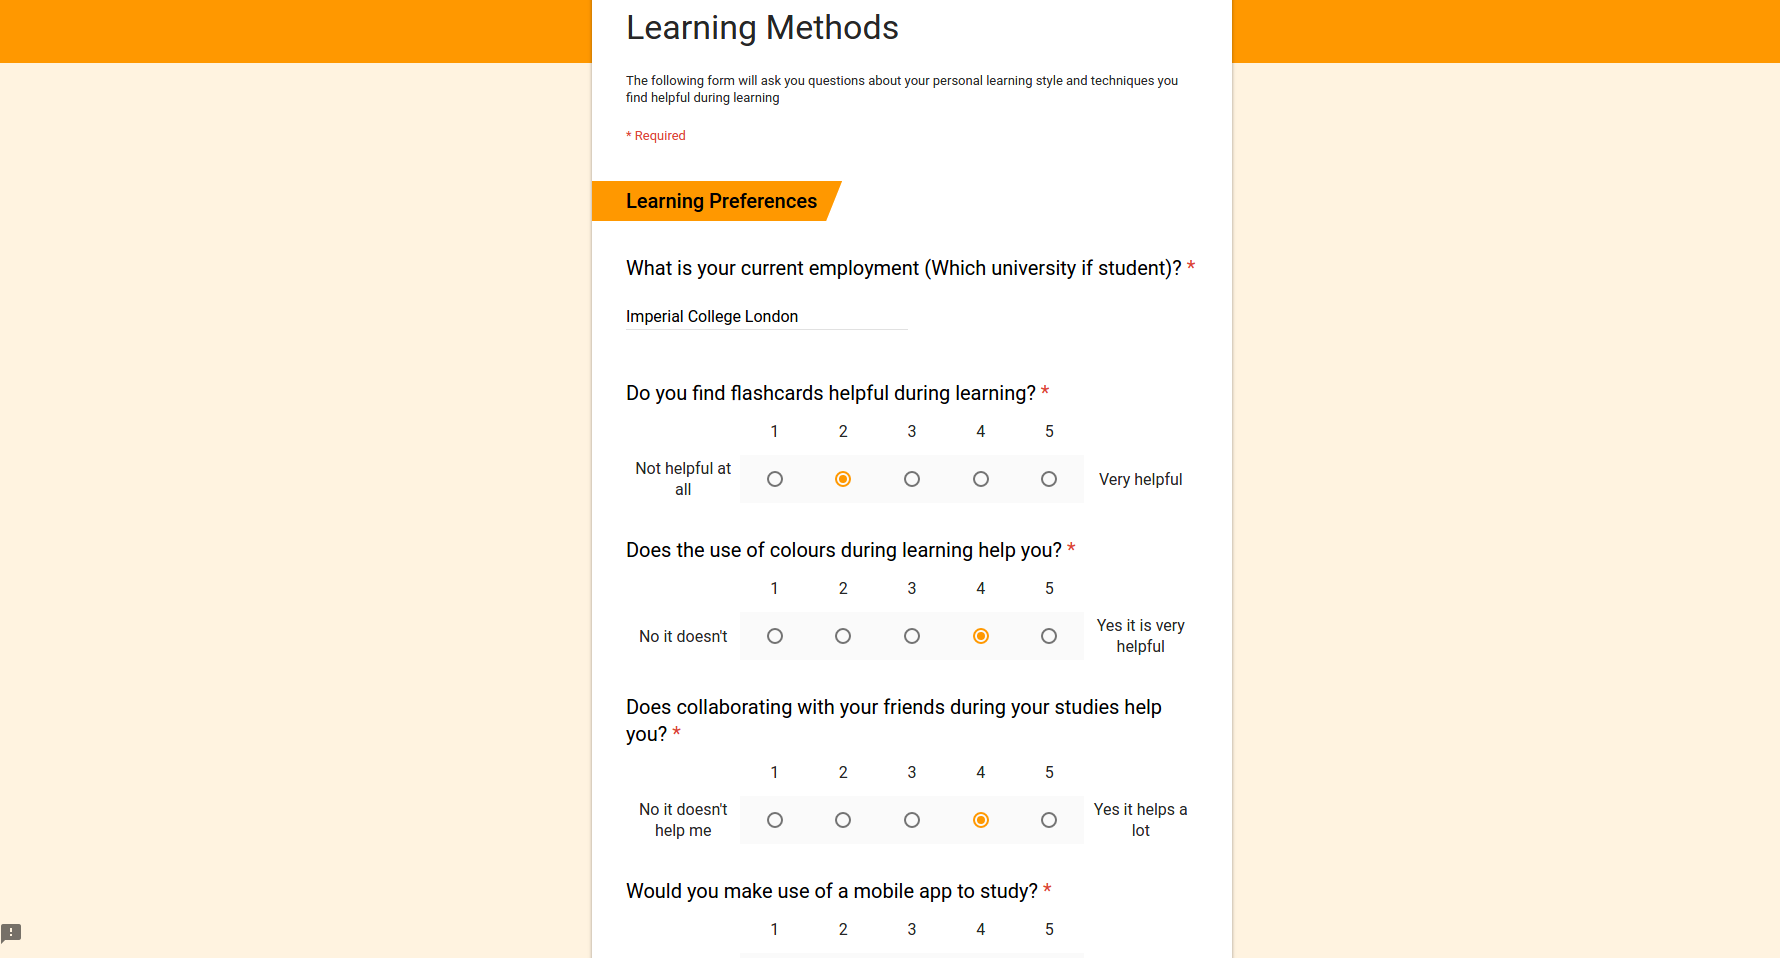
\includegraphics[scale=0.14]{form.png}
	\vspace{1mm}
\end{center}

Using the Google form above, we surveyed our friends, their friends and then their friends as part of our market research.  This meant we didn't just get opinions from Imperial College, but from all parts of the UK like Scotland and Northern Ireland.  It gave us the following results:

\begin{figure}[ht]
	\centering
	\begin{subfigure}{}
	  \centering
			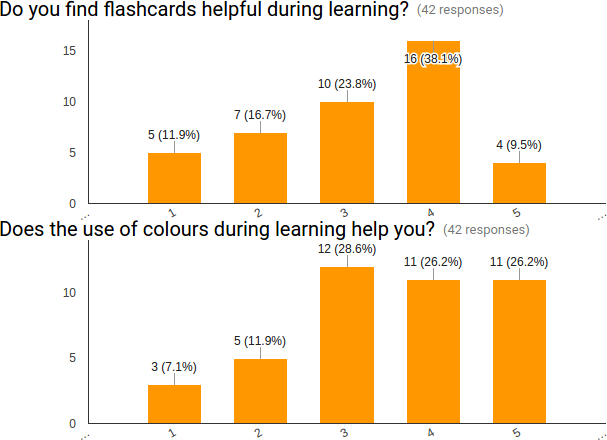
\includegraphics[width=5.85cm, height=5.8cm]{images_colours.png}
	\end{subfigure}%
	\begin{subfigure}{}
	  \centering
			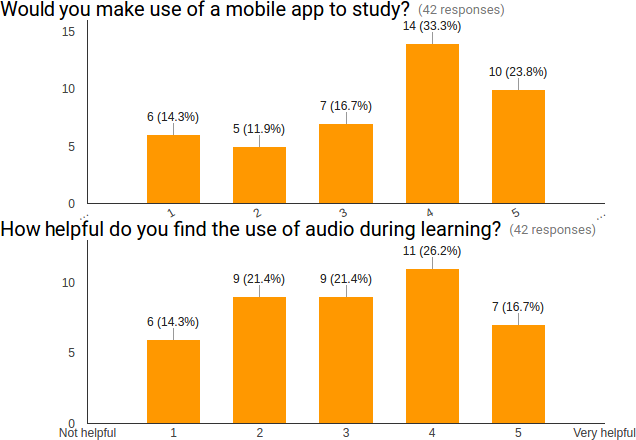
\includegraphics[width=5.85cm, height=5.8cm]{mobile_audio.png}
	\end{subfigure}
\end{figure}

\newpage
More importantly it gave the users a chance to say what they have problems with during revision and what they would like to see to combat it.

\begin{center}
	\vspace{1mm}
	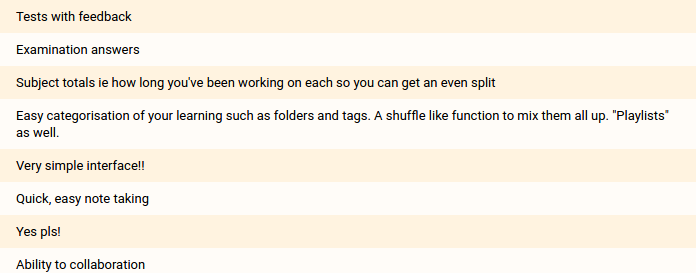
\includegraphics[scale=0.5]{feedback.png}
	\vspace{1mm}
\end{center}

We then took these general problems and asked some people around us to expand on this and what the core problems they had were.

The answers we got we that revision notes were too much for one person to handle and that it is hard to test yourself easily and properly on said notes.
We then wanted to investigate this further and how many collaboration of flashcards could help form a solution to this.

We read papers on group work saying that groups "can save time and requires a shared workload" \cite{groupwork1} and "people remember group discussions better" \cite{groupwork2}. We thought this was a key idea and decided that collaboration would drive our process forward.


\begin{thebibliography}{2}
	\bibitem{groupwork1} 
		\url{https://sydney.edu.au/education_social_work/groupwork/docs/BenefitsOfGW.pdf}
	\bibitem{groupwork2} 
		\url{http://uncw.edu/cte/et/articles/Vol11_2/Burke.pdf}
\end{thebibliography}

\end{document}